\noindent
Visualization not only covers the graphical representation of things (\eg
molecules, measurement data, \dots) but also the graphical user interface
(GUI). Both jobs can be done using \class{VIEW} functionality. Both areas are
discussed in the next few sections.

\section{Modularity}
In general most of the time in GUI programming is spent on implementing the 
interactions of the individual elements of the user interface with each other 
(\eg defining menu entries, button actions, etc.). In order to reduce these 
efforts, the functionality in the VIEW library has been bundled into different
modules (\eg OpenGL rendering, force field methods, the scripting language 
interface, etc.), which can be freely combined to an application. These modules
automatically connect to each other and thus allow the user to add further 
functionality with as little as a single line of code. To this end, we have 
designed a set of  base classes describing the interactions of the interface 
elements. The two most important components in this design are 
\class{MainControl}, the application's main window, and 
\class{ModularWidget}, the base class for all modules.
The next pages will describe the modeling and implementation of this approach.
\label{modularity}

\paragraph{MainControl} 
\hspace*{\fill}\\
The class \class{MainControl} is derived from Qt's \class{QMainWindow} and thus
realizes an application's main window. It contains only the most essential data
structures: The \class{CompositeManager} stores all molecular entities
(\class{Composite} objects) and the \class{PrimitiveManager} is responsible for
the representations (\ie geometric models) and the thread for their
(re)calculation. All additional functionality (\eg reading and writing of 
structures, OpenGL visualization, etc.) are added to the main window by 
instantiating one of the classes derived from \class{ModularWidget}. 

\paragraph{Modular Widgets}
\hspace*{\fill}\\
\class{ModularWidget} is a common base class for all the modules, that can be
combined to form an entire application. While the modular widgets are widely 
independent, they can still notify each other about the current work flow. 
This is achieved by a messaging system, that allows a \class{ModularWidget}
to send a message which is then received by all other modular widgets (see 
Section~\ref{message}).
\\
In addition to the messaging system, the \class{ModularWidget} class provides 
many other commonly needed features to ease and accelerate the development of
new modules:
\begin{itemize}
%\item Sending and receiving of messages
\item Showing status and error messages
\item Management of menu and toolbar entries 
\item Registering widgets and menu entries for the help system
\item Management of preferences dialogs
\item Reading/writing of settings from/to a configuration file
\item Registering of supported file formats e.g.\ for parsing command line arguments
or drag-and-drop support
\item Access to individual instances with the method \class{getInstance()}
\item Access to the \class{MainControl} and thus to the loaded molecules and representations
\item Locking of molecular entities while multithreaded code is running
\end{itemize}

For many different tasks (see Table \ref{table:tmw}),
the VIEW library already contains a wide variety of modular widgets.
Since they are widely independent from each other, they can easily
be combined to an application. All that is needed, is the instantiating
of modular widgets with the \class{MainControl} as their parent, as can be seen in
the following code snippet:
\begin{lstlisting}{}
  Mainframe::Mainframe(...)
   : MainControl(...)
  {
    new LogView(this);          // widget (1)
    new DatasetControl(this);   // widget (2)
    new PyWidget(this);         // widget (3)
    new MolecularControl(this); // widget (4)
    new GeometricControl(this); // widget (5)
    new Scene(this);            // widget (6)
  }
\end{lstlisting}

These few lines of code (header includes were omitted for brevity) create a fully-fledged 
molecular structure viewer.
In addition to using already existing widgets, users can easily implement new ones,
especially since \class{ModularWidget} already offers many common features (see above).
As a result, users can freely combine new and existing widgets both 
to extend BALLView with new functionality or to create entirely new custom-tailored 
applications.

\begin{table} [ht] %[htbp]
\centering
\begin{tabular} {|l|l|}
\hline
\bf Name& \bf Functionality\\
\hline
\class{DatasetControl}& Management of data sets\\
\class{DisplayProperties}& Creation and modification of models\\
\class{DockingController}& Molecular docking\\
\class{DownloadPDBDialog}& Downloads from the protein database\\
\class{EditableScene}& Molecular editing\\
\class{FDPBDialog}& Calculation of electrostatic potentials\\
\class{FileObserver}& Observing changes in a molecular file\\
\class{GeometricControl}& Management of graphical representations\\
\class{LabelDialog}& Creation of labels in the 3D view\\
\class{LogView}& Logging window\\
\class{ModifyRepresentationDialog}& Custom colorings for models\\
\class{MolecularControl}& Hierarchical overview of loaded molecules\\
\class{MolecularFileDialog}& Reading and writing of molecular files\\
\class{MolecularStructure}& Force field and molecular mechanics features\\
\class{PyWidget}& Python scripting\\
\class{Scene}& three-dimensional graphics\\
\class{SnapshotVisualisationDialog}& Visualization of trajectories\\
\class{TestFramework}& Recording and playback of user input\\
\hline
\end{tabular}
\caption[Overview on the derived modular widgets]
{Overview of the classes derived from \class{ModularWidget}. 
Each individual class was created for one specific domain of features and is widely 
independent from the other widgets.
}
\label{table:tmw}
\end{table}


\paragraph{Example for the implementation of a modular widget}
\hspace*{\fill}\\
To visualize how new modular widgets can be created, the following pages will outline 
the implementation of the class \class{LabelDialog}, which is
part of the VIEW library. 
Its purpose is to create labels in the 3D view for a list of 
highlighted molecular entities and it has the following capabilities:
The menu entry {"Add Label"} toggles the dialog's visibility and is 
disabled if no molecular entities are highlighted in the \class{MolecularControl}.
When the dialog is shown, the user can select a font and its color, the desired text for 
the label(s), and choose if only one label is to be created for the entire selection or 
one label for every atom/residue.  
When the "Apply" button is pressed, a new \class{Representation} is created with the newly 
created label(s).
For convenience the chosen color and font are stored in the application's configuration 
file for future usage.
\\ 
\\
The dialog's layout was done with the program "Qt Designer" (see ~\ref{designer}).
This results in a source file, containing the base class \class{Ui\_LabelDialogData}, which 
defines the dialog's layout. The actual dialog class is derived from this layout class.
This procedure accelerates the development process and makes the dialog's 
layout independent from its function.
The following code is the content of the header file for the actual dialog.
The includes, namespaces, and some documentation lines were omitted for brevity and the
overloaded methods from the \class{ModularWidget} base class were marked.
\begin{lstlisting}{}
class BALL_VIEW_EXPORT LabelDialog 
  : public QDialog,
    public Ui_LabelDialogData,
    public ModularWidget
{
  // macro needed for Qt's slot mechanism:
  Q_OBJECT

  // Macro from the Embeddable class:
  BALL_EMBEDDABLE(LabelDialog,ModularWidget)
	
  public:
  LabelDialog(QWidget *parent = NULL, const char *name = NULL );
  virtual ~LabelDialog();
					
  // method for message handling, overloaded from ModularWidget
  virtual void onNotify(Message* message);
					
  // method for reading settings, overloaded from ModularWidget
  virtual void fetchPreferences(INIFile &inifile);
  // method for written settings, overloaded from ModularWidget
  virtual void writePreferences(INIFile &inifile);
		
  // method for e.g. initializing menu entries, overloaded from ModularWidget
  virtual void initializeWidget(MainControl& main_control);

  // Overloaded from ModularWidget
  virtual void checkMenu(MainControl& main_control);
	
  protected slots:
  virtual void accept();
  virtual void editColor();
  virtual void addTag();
  virtual void fontSelected();
  virtual void modeChanged();
  void textChanged();

  protected:
  Representation* createOneLabel_();
  Representation* createMultipleLabels_();
  QAction*    menu_entry_;
  ColorRGBA   custom_color_;
  QFont       font_;
};
\end{lstlisting}

The following paragraphgraphs will discuss the actual implementation, starting with the 
constructor: It must be called with the \class{MainControl} as parent to enable the 
registration of the \class{ModularWidget}.
Since this example class is derived from three other classes, these also have to
be initialized. 
The function \class{setupUi} stems from the ''*.ui' file and defines the layout of the dialog.
Next the individual buttons and check boxes are connected to their slots.
The call of \class{registerWidget} is of special importance since it enables the internal 
mechanism that connects all modular widgets with each other (i.e.\ the messaging system).
\begin{lstlisting}{}
LabelDialog::LabelDialog(QWidget* parent, const char* name)
  :  QDialog(parent),
     Ui_LabelDialogData(),
     ModularWidget(name)
{
  // apply the dialogs layout:
  Ui_LabelDialogData::setupUi(this);

  // signals and slots connections
  connect(apply_button_, SIGNAL(clicked()), this, SLOT(accept()));
  connect(buttonCancel, SIGNAL(clicked()), this, SLOT(reject()));
  connect(edit_button, SIGNAL(clicked()), this, SLOT(editColor()));
  connect(add_tag_button, SIGNAL(clicked()), this, SLOT(addTag()));
  connect(font_button, SIGNAL(clicked()), this, SLOT(fontSelected()));
  connect(all_items, SIGNAL(toggled(bool)), this, SLOT(modeChanged()));
  connect(text_box, SIGNAL(editTextChanged(const QString&)), 
              this, SLOT(textChanged()));

  setWindowTitle("Add Label");
  setObjectName(name);
  hide();

  // register the widget with the MainControl
  ModularWidget::registerWidget(this);
}
\end{lstlisting}

All modular widgets can have their own menu entries in the applications menu bar.
These entries should be initialized in the virtual method 
\class{initializeWidget}, which will be automatically called by the \class{MainControl}
for all registered \class{ModularWidget} subclasses.
For this concrete class, the method creates the menu entry "Add Label" and connects 
it to a slot, which will open the dialog. 
The creation of the menu entry is done through a call of \class{insertMenuEntry}, 
which will also create the given menu (if it does not yet exist) and return a pointer to 
a \class{QAction}. 
This pointer is then assigned to the variable \class{id\_}, which will later be used for 
enabling and disabling the menu entry.
Corresponding to the method \class{initializeWidget} exists the \class{initializePreferencesTab} method to add sub pages to the applications preferences dialog. 
Since this dialog does not have a configuration dialog, this function is not needed in 
the \class{LabelDialog} class.
\begin{lstlisting}{}
void LabelDialog::initializeWidget(MainControl& main_control)
{
  menu_entry_ = ModularWidget::insertMenuEntry(
                  MainControl::DISPLAY, "Add Label", this, SLOT(show()));
  setMenuHint("Add a label for selected molecular objects");   
}
\end{lstlisting}

\vspace{-0.2cm}
The next method \class{onNotify} does the message processing:\label{onNotify}
It is overloaded from the \class{ModularWidget} class and gets called when a \class{Message} 
arrives for the widget. In the \class{LabelDialog} class, it does the following:
If no molecular entities are highlighted in the \class{MolecularControl}, the dialog's 
"Apply" button is disabled and the menu entries are checked if they have to be 
enabled/disabled. 
This is done to ensure, that the dialog can not be used while e.g.\ a simulation is 
running, since the molecular entities could changed at any time. 
This is checked in the \class{checkMenu} method with a call to \class{MainControl::isBusy()}, 
which returns true if a modular widget locked the molecular entities because they could 
be changed or if an model update is underway.
\begin{lstlisting}{}
void LabelDialog::onNotify(Message* message)
{
  ControlSelectionMessage* sm = 
    RTTI::castTo<ControlSelectionMessage>(*message);

  if (sm != 0)
  {
    // disable apply button, if selection is empty
    apply_button_->setEnabled(!sm->getSelection().empty();
    checkMenu(*getMainControl());
  }
}

void LabelDialog::checkMenu(MainControl& mc)
{
  Size selection_size = mc.getMolecularControlSelection().size();
  menu_entry_->setEnabled(selection_size && !mc.isBusy());
}
\end{lstlisting}

The following methods are only of minor interest and just shown for the sake of completeness.
They are called when a user clicks on the
corresponding buttons and perform auxiliary functions, like choosing the label's 
font or color.
\begin{lstlisting}{}
void LabelDialog::editColor()
{
  custom_color_.set(chooseColor(color_sample_));
}

void LabelDialog::addTag()
{
  QString tag;
  if (tag_box->currentText() == "Name")                tag = "%N";
  else if (tag_box->currentText() == "Residue ID")     tag = "%I";
  else if (tag_box->currentText() == "Atom Type")      tag = "%T";
  else if (tag_box->currentText() == "Atom Charge")    tag = "%C";
  else if (tag_box->currentText() == "Atom Type Name") tag = "%Y";
  else if (tag_box->currentText() == "Element")        tag = "%E";

  text_box->lineEdit()->setText(text_box->currentText() + tag);
}

void LabelDialog::fontSelected()
{
  bool ok = true;
  QFont font = QFontDialog::getFont(&ok, font_, 0);
  if (!ok) return;

  font_label->setFont(font);
  font_ = font;
}

void LabelDialog::modeChanged()
{
  tag_box->setEnabled(!all_items->isChecked());
  add_tag_button->setEnabled(!all_items->isChecked());
}

void LabelDialog::textChanged()
{
  apply_button_->setEnabled(text_box->currentText() != "");
}
\end{lstlisting}

\vspace{0.5cm}
When a user presses the dialog's "Apply" button, the method \class{accept()} is called.
It does the actual label creation and adds the label(s) to the 3D view:
First the current list of highlighted molecular entities is obtained from
the \class{MainControl}.
Then a \class{LabelModel} processor is created and added to a \class{Representation}.
Next the values from the dialog are applied to the \class{LabelModel} and the
list of molecular entities is stored in the \class{Representation}.
This approach may seem a bit complex but it has a distinct advantage: The position
of the label will be automatically updated if the 3D positions of the molecular entities 
should change. 
Finally the \class{Representation} is stored in the \class{MainControl} and it is rendered
in the 3D view with a call of \class{MainControl::update(Representation\&)}.
The methods in the \class{MainControl} for inserting and updating representations were 
added just for convenience reasons and contain only the code for sending the corresponding 
messages. 
As an example, \class{MainControl::insert(Representation\&)} only consists of the 
following code:
\begin{lstlisting}{}
  notify_(new RepresentationMessage(representation, 
                                    RepresentationMessage::ADD));
\end{lstlisting}

After the last modular widget was notified, the message will be automatically deleted.
Therefore messages, that are about to be send, have to be created on the heap.
\begin{lstlisting}{}
void LabelDialog::accept()
{
  List<Composite*> selection = 
    getMainControl()->getMolecularControlSelection();

  // no selection present => return
  if (selection.empty()) return;

  Representation* rep = new Representation;
  rep->setProperty(Representation::PROPERTY__ALWAYS_FRONT);
  rep->setModelType(MODEL_LABEL);

  LabelModel* model = new LabelModel;
  model->setText(ascii(text_box->currentText()));
  model->setColor(custom_color_);
  model->setFont(font_);

       if (    all_items->isChecked()) model->setMode(LabelModel::ONE_LABEL);
  else if (   every_atom->isChecked()) model->setMode(LabelModel::ALL_ATOMS);
  else if (every_residue->isChecked()) model->setMode(LabelModel::ALL_RESIDUES);
  else if (   every_item->isChecked()) model->setMode(LabelModel::ALL_ITEMS);

  rep->setModelProcessor(model);

  // process all objects in the selection list
  List<Composite*>::ConstIterator list_it = selection.begin();
  List<const Composite*> composites;
  for (; list_it != selection.end(); ++list_it)
  {
    composites.push_back(*list_it);
  }

  rep->setComposites(composites);
  getMainControl()->insert(*rep);
  getMainControl()->update(*rep);
  text_box->addItem(text_box->currentText());
  setStatusbarText("Label added.");
}
\end{lstlisting}

The next two methods are responsible for reading and writing the of this widget's settings.
The first method, \class{fetchPreferences}, restores the settings from the configuration file.
If the this file has a section with the name \class{WINDOWS} and a key 
''\class{Label::customcolor}'' within, then the content of this key is read and converted 
to a color, which is then assigned to the dialog's label and stored in the variable
\class{custom\_color\_}.
\begin{lstlisting}{}
void LabelDialog::fetchPreferences(INIFile& inifile)
{
  // restore the color 
  if (inifile.hasEntry("WINDOWS", "Label::customcolor"))
  {
    custom_color_.set(inifile.getValue("WINDOWS", "Label::customcolor"));
    setColor(color_sample_, custom_color_);
  }

  // restore the font
  if (inifile.hasEntry("WINDOWS", "Label::font"))
  {
    font_.fromString(inifile.getValue("WINDOWS", "Label::font").c_str());
  }
  font_label->setFont(font_);
}
\end{lstlisting}

\vspace{0.3cm}
To write all user defined options in a configuration file, the method
\class{ModularWidget::writePreferences} was overridden:
\begin{lstlisting}{}
void LabelDialog::writePreferences(INIFile& inifile)
{
  ModularWidget::writePreferences(inifile);

  // store the color
  inifile.insertValue("WINDOWS", "Label::customcolor", custom_color_);
  // store the font
  inifile.insertValue("WINDOWS", "Label::font", ascii(font_.toString()));
}
\end{lstlisting}

This concludes the implementation of the \class{LabelDialog} class. 
It can be used in a derived \class{MainControl} class, simply by adding the following line: 
\begin{verbatim}
	new LabelDialog(this, "LabelDialog");
\end{verbatim}
This one line of code is all that is needed to make the dialog work, all needed function 
calls inside the \class{LabelDialog} class will be automatically done by the VIEW framework.
\\
\\
This example demonstrates, how effective the encapsulation of features into distinct
modules works: Since the modules are mostly independent from each other and the interface
base classes take care of all basic functions, it is very easy to extend the application
with new features.

\section{Messaging system} \label{message}
A special mechanism was needed for allowing the individual modular widgets to be mostly 
independent from each other but still be able work together i.e.\ by notifying each other 
about the current work flow. 
This was achieved by a messaging system, that allows a \class{ModularWidget} to send a 
message which is then received by all other modular widgets.
As an example: 
The \class{MolecularControl} provides a hierarchical overview of the loaded molecules
and notifies the other widgets when a user highlights some of its entries. 
This is needed, since other modular widgets offer tool bar entries for features (like 
saving molecules) that operate on the currently highlighted objects. 
These entries get disabled if no molecular item is highlighted.
To notify the other widgets, the \class{MolecularControl} sends a \class{ControlSelectionMessage}
which is then received by the \class{MolecularFileDialog}.
This class provides the functionality for loading and writing molecular files and will 
then disable the corresponding menu and toolbar entries.\\
Since the modular widgets have to notify each other about many different events, the class
\class{Message} has many subclasses (see Table~\ref{tab:messages}), which store different data
types, like selections or object pointers. 
If a new event is introduced, it can easily be added by creating an other \class{Message} 
subclass.
\\
The actual sending of messages is done in the method \class{ModularWidget::notify\_}, while 
the message is received by \class{ModularWidget::onNotify()} (for an example of a concrete
implementation see page~\pageref{onNotify}).
In this method the modular widget has to decide if it needs to react to the message. 
This is in general done by using runtime type identification. 
In addition, many different messages also provide enumeration values for defining further
specialized message subtypes. 
A \class{CompositeMessage} can e.g.\ cope with the events of an added or deleted 
\class{Composite} by using the types \class{CompositeMessage::NEW\_COMPOSITE} or 
\class{CompositeMessage::REMOVED\_COMPOSITE}.
The usage of these enumeration subtypes has the advantage, that much less subclasses
are needed to distinguish different classes of events, resulting in a slimmer implementation.
Thus we only added new \class{Message} subclasses, when a message had to transmit a new kind 
of data, or if no appropriate class yet existed.
%-- Anordnung der Casts entsprechend der auftretenden Hauefigkeit der Nachricht\\
%The current implementation has a small drawback: Since all modular widgets receive a message
%the method onNotify() may be called many times in a row. 
\begin{table} [ht] %[htbp]
\centering
\begin{tabular} {|l|l|}
\hline
CompositeMessage & SceneMessage\\
GenericSelectionMessage & ControlSelectionMessage\\
NewSelectionMessage & GeometricObjectSelectionMessage\\
RepresentationMessage & MolecularTaskMessage\\
ShowDisplayPropertiesMessage & CreateRepresentationMessage\\
RegularDataMessage & RegularData1DMessage \\
RegularData2DMessage & RegularData3DMessage\\
NewDockResultMessage & NewTrajectoryMessage\\
ShowDockResultMessage & DockingFinishedMessage\\
DeselectControlsMessage & \\
\hline
\end{tabular}
\caption{Derived message classes. 
All the individual classes can contain specific datas and some have an addition enumeration 
type to differ between subtypes of messages.}
\label{tab:messages}
\end{table}
%
\section{Design of the visualization classes}
\paragraph{Geometric objects}
\hspace*{\fill}\\
\label{geometric_objects}
We created a base class \class{GeometricObject} to provide a general interface for geometric 
shapes, that can be calculated and rendered in the VIEW framework. 
From this base class, we then derived the classes for the individual tangible geometric 
objects (see Table~\ref{tab:go}).
The instances of these derived classes are created by the different model processors and 
later get colored by the color processors, and stored in a \class{Representation}. 
The renderer classes can then translate their informations such that they can e.g.\ be 
drawn on the screen or processed by an external program.
\begin{table} [ht] %[htbp]
\centering
\begin{tabular} {|l|l|}
\hline
Box & Disc\\
Label & GridVisualisation\\
Mesh & QuadMesh\\
Point & SimpleBox\\
Sphere & Tube\\
Line & TwoColoredLine \\
Tube & TwoColoredTube\\
IlluminatedLine& \\
\hline
\end{tabular}
\caption{Overview of the different geometric objects that are supported in the VIEW 
	framework.}
\label{tab:go}
\end{table}

We created numerous derived \class{GeometricObject} classes, to guarantee that virtually
all thinkable shapes and objects can be visualized. 
If nevertheless in the future the need for a new kind of geometric object would arise, 
this could be realized with minimal effort:
All that would have to be done, is to create a new derived \class{GeometricObject} class and 
add the corresponding rendering methods to the \class{Renderer} classes 
(see Page~\pageref{renderer}).

\label{representation}
\paragraph{Representations}
\hspace*{\fill}\\
To offer the user an intuitive way of handling models and their coloring,
we created the class \class{Representation}. 
For each visualized object, this class stores the selection of molecular entities, the used 
model and coloring method, the drawing style, and the geometric objects representing the 
model (see Fig.~\ref{fig:representation}).
This approach has many advantages:
\begin{itemize}
\item 
The different models and coloring methods can be freely combined.
\item
Users can can create customized representations e.g. by using the Python scripting interface.
\item
Users can combine as many different representations as they like to compose complex molecular visualizations.
\item
Individual representations can be enable/disable any time.
\item
It is possible to write project files, which store all representations for later usage.
\item
A \class{Representation} can easily be redrawn, when the corresponding atoms have changed.
\item
A user can disable all updates to a representation
e.g.\ to visualize the differences between two steps in a trajectory.
\end{itemize}

We wanted to make the creation and modification of representations as easily as possible.
Thus we designed a user friendly dialog, which can assign all
the different settings of a \class{Representation}.\\
The classes \class{ModelProcessor} and \class{ColorProcessor} which are responsible 
for creating the different models and coloring schemes are described in the
section below.
\begin{figure*}[ht] %[htbp]
\centering
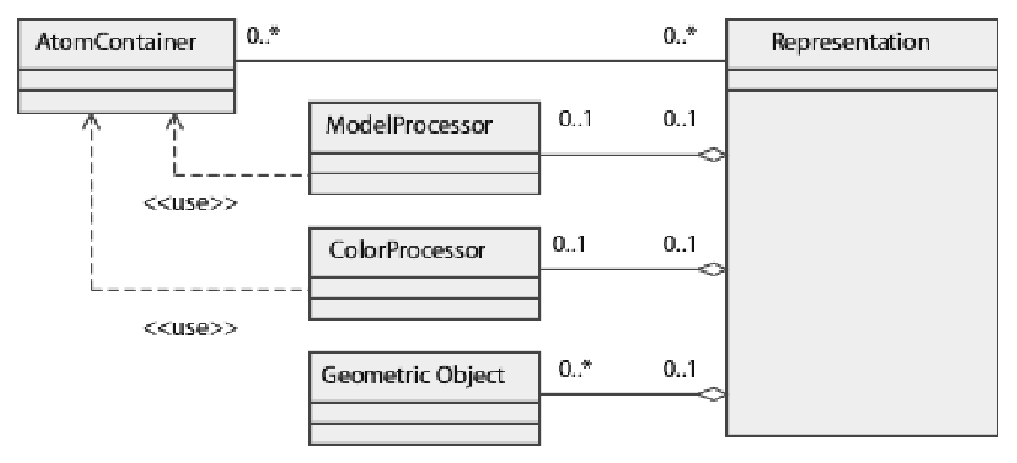
\includegraphics[width=1.\textwidth]{representation.eps}
\caption[UML diagram for the \class{Representation} class]
{Each visualized object corresponds to an instance of the class 
\class{Representation}. The \class{ModelProcessor} creates 
\class{GeometricObjects}, \eg tubes or meshes for all atoms stored in the
\class{AtomContainers}. Next, the \class{ColorProcessor} colorizes the 
\class{GeometricObjects}, e.g.\ by element, charge or temperature factor. The
individual model types and coloring methods are realized by derived classes.
This approach simplifies the creation of new models and coloring methods and 
allows their free combination.}
\label{fig:representation}
\end{figure*}

\paragraph{Models and Coloring}
\hspace*{\fill}\\
We created a wide variety of different models.
All these model classes are derived from the \class{ModelProcessor}.
This class is again derived from the BALL class \class{UnaryProcessor$<$Composite$>$}, 
which provides a general interface for recursively iterating and processing a 
\class{Composite} tree.
Therefore a \class{ModelProcessor} can be be applied to entire proteins as well as on 
individual atoms, which makes it is easily possible to create models for user defined 
subselections of molecules.
When a model processor is applied to such a selection, it first iterates over the
\class{Composite} tree and collects the information necessary for the model's creation.
With this information, the method \class{createGeometricObjects()} can then create the 
individual geometric object, which form the model. 
The geometric objects are created on the heap and stored in a list inside the 
\class{Representation}, which is then responsible for deleting them.
\\
The counterpart to \class{ModelProcessor} is \class{ColorProcessor}, which iterates over a 
list of \class{GeometricObjects} and finds the corresponding color for each one.
Currently 16 different coloring methods are implemented and
every single one is derived from \class{ColorProcessor}.
\\
Since users directly perceive on how long it takes to create a representation,
we made great efforts to ensure maximum performance for the model and coloring 
calculations.

\paragraph{Renderer}\label{renderer}
\hspace*{\fill}\\
Currently BALLView support two different renderer: Real time graphics are provided by the
OpenGL renderer (\class{GLRenderer}) while high quality graphics are available through the 
POVRay exporter (\class{POVRenderer}).
Both classes are derived from a common base class \class{Renderer}, which provides a general 
interface.
This ensures, that in future versions, arbitrary renderer can easily be added by
deriving a further class from \class{Renderer}.
The actual rendering of a \class{Representation} is done in the method
\class{Renderer::render(const Representation\&)}.
It iterates over all geometric objects in the \class{Representation} and,
by using runtime type identification, finds the corresponding rendering method:
\begin{lstlisting}{}
  if      (RTTI::isKindOf<Point>(*go)) renderPoint_(*(const Point*) go);
  else if (RTTI::isKindOf<Disc>(*go))  renderDisc_( *(const Disc*)  go);
  else if (RTTI::isKindOf<Line>(*go))  renderLine_( *(const Line*)  go);
\end{lstlisting}
 
These methods are overridden in the derived classes with the real rendering
code, \eg OpenGL calls in the \class{GLRenderer}. 
This approach ensures that the different renderer can easily be extended with support for 
new kinds of geometric objects, simply by adding a new rendering method and an appropriate 
runtime check.
\\
\\
Unlike the OpenGL renderer, the \class{POVRenderer} does not provide real time graphics,
but an interface to the external POVRay renderer.
To do so, it translates the data in the geometric objects to a form that can be 
parsed by the POVRay application. 
The resulting text is then written to an output stream, which is either a
file or the standard console output.

\section{Creating dialogs}
\label{designer}
To layout the dialogs in the VIEW library, we used the program "Qt Designer".
It is part of every Qt-package and provides a comfortable "What you see is what you get"
(WYSIWYG) interface for designing widgets.
The result of the "Qt Designer" program is a ".ui" file, which is then transformed 
into a set of C++ source files by the Qt program "uic".
These source files contain a base class, which defines the dialog's layout . 
The actual dialog class will be derived from the layout class and contains the dialog's
actual functionality.
\\
While this procedure may seem a bit complicated, it is actually straightforward and 
very useful:
Not only does the "Qt Designer" WYSIWYG interface accelerates the development process, 
the resulting "*.ui" files also uncouple the dialogs' layout from its function. 
Thus a software engineer can extend the functionality without 
having to care about the dialog's layout, while a GUI designer can change the layout
without the need to adapt the source code.

\section{User defined settings}
\label{preferences}
We wanted to give BALLView's users the opportunity to adapt it to their liking in any
thinkable way, including the different models, coloring methods, and display options. 
Therefore an extensible graphical user interface was needed for applying these settings. 
For this purpose, we developed the \class{Preferences} dialog, which can contain an 
arbitrary number of child dialogs. 
These child dialogs are stored in a \class{QWidgetStack} and shown as entries in 
a hierarchical list. 
If a user clicks on such an entry, the corresponding dialog is then shown in the 
widget stack.
This approach allows to cluster the different settings in a hierarchical way
and users can freely browse and apply the individual settings.
Furthermore the \class{Preferences} dialog can have any number of child dialogs and still 
have a concise layout.
In an earlier implementation, we used a tab widget, which is the standard approach for
such dialogs. This solution proved to be less suited, since the child dialogs can not
be clustered and the layout becomes unhandy, if many children are added.

\paragraph{Automation of the (re)storing process}
\hspace*{\fill}\\
All the settings, that can be adapted in the \class{Preferences} dialog, shall be 
stored when BALLView is closed.
To this end all configuration dialogs have to store the content of their GUI elements,
like line edits or check boxes.
In the early versions of our implementation, every dialog provided its
own routines for this purpose.
Since this created a lot of overhead in means of redundant source code,
we wanted to automate the (de)serialization:
We designed a base class \class{PreferencesEntry}, which can act as a base class for any dialog.
It automatically registers a dialog's GUI elements, whose content is then later
saved or restored.
All that is now needed, is to add one line of code in the 
the dialog's constructor:
\begin{lstlisting}{}
  registerWidgets_();
\end{lstlisting}

This sole line ensures, that the dialog's data get stored or read.
Compared to the earlier implementation, which often had dozens of lines
for this task, this is an essential improvement.

\paragraph{The storing process}
\hspace*{\fill}\\
To store the content of the registered GUI elements, their content
is transformed into a string (see below) which is later written to the configuration
file along with the name of the GUI element.

\begin{lstlisting}{}
  if (RTTI::isKindOf<QLabel>(*widget))
  {
  	value = getColor(dynamic_cast<const QLabel*>(widget));
  }
  else if (RTTI::isKindOf<QLineEdit>(*widget))
  {
    value = ascii((dynamic_cast<const QLineEdit*>(widget))->text());
  }
  else if (RTTI::isKindOf<QCheckBox>(*widget))
  {
    value = String((dynamic_cast<const QCheckBox*>(widget))->isChecked());
  }
\end{lstlisting}

The resulting configuration file is line based and divided into sections,
which can correspond to individual dialogs. The following lines illustrate
the section for the dialog that configures and starts energy minimization runs.
From these lines the whole content of the dialog can be reconstructed and thus the 
minimization settings restored.
\begin{lstlisting}{}
  [MINIMIZATION]
  energy_difference_lineedit=0.0001
  max_iterations_lineedit=100
  refresh_iterations_lineedit=25
  minimization_group=conjugate_button
  max_grad_lineedit=1.000000
\end{lstlisting}

\paragraph{Further extensions}
\hspace*{\fill}\\
Since the described approach for storing the content of dialogs turned out to be very 
effective, we extended its usage. 
Now, dialogs no longer have to be child widgets in the 
\class{Preferences} dialog, to use this feature.
%Thus e.g.\ the dialogs for the setup of the individual forcefields can 
In addition, the \class{PreferencesEntry} class now also supports the storing of default 
values, that are applied when a dialog's ''Defaults'' button is pressed.
In just the same way a dialog gets restored to its originally values, when the ''Cancel'' 
button is pressed.\\
\\
An other extension was made to support more sophisticated
GUI elements: We created a base class \class{ExtendedPreferencesObject}, that defines an 
interface for (re)storing the content of composite widgets, like e.g. the tables for the 
setup of the different coloring methods. This approach further improves the 
extensibility, since new, derived \class{ExtendedPreferencesObject} classes can be designed
and added.
What is even more important: Compared to a basic implementation, the described approach is also much less error-prone, since a developer 
can no longer accidentally forget to add the (re)storing code for one GUI element.

\paragraph{Summary}
\hspace*{\fill}\\
We designed a very user-friendly way to apply any arbitrary number of options. 
In addition, the implemented approach is also very handy for developers, since it
is very extensible and minimizes the efforts for (re)storing the content of further dialogs. 
\\
\\
The VIEW library in its current state has more than 20 dialogs, whose content is (re)stored. 
These dialogs have in total more than 200 widgets that contain user defined data.
A conservative estimation of 8 lines of code per widget for the storing/restoring of its data, results in 
the saving of more than 1500 lines of code.
%%%%%%%%%%%%%%%%%%%%%%%%%%%%%%%%%%%%%%%%%%%%%%%%%%%%%%%%%%%%%%%%%%%%%%%%%%%%%%%%%%%%%%
\section{Multithreading}\label{mthread}
%Since a responsive interface is critical, even while CPU intensive processing tasks are running,
Molview, the precursor of BALLView was designed as a single-threaded application. 
As a result, the graphical user interface would freeze, while a calculation like a 
molecular dynamics simulation was running.
Therefore users could no longer interfere with the application.
This was especially tiresome since the calculations could not be aborted, except by 
shutting down the entire program.
To circumvent these limitations, we had to redesign the VIEW library to use mulithreading 
techniques.
Now all long running calculations like MD simulations and energy minimizations are 
started in their own thread.
This has several advantages:
\begin{itemize}
\item The user interface stays responsive at any time and may thus e.g.\ print estimated run times.
\item Multithreaded calculations can be stopped with the ease of one mouse click.
\item The 3D graphics widget can be used to show intermediate results e.g.\ while a minimization is running.
\item Users can reposition the viewpoint e.g.\ to focus on one functional group while a MD simulation is running.
\item Multiple threads can make efficient use of multi-processor or multi-core computers.
\end{itemize}
Since multithreading has so many advantages, we also used it for further purposes:
The (re)calculation of models and colorings are now also started in separagraphte threads.
A further functionality were the mulithreading technique became very handy is the dialog for 
downloading structures from the protein database. 
Here it allows to monitor the progress of the download and to abort it at any time.

\paragraph{Locking data structures and synchronization of threads}
\hspace*{\fill}\\
Unfortunately multithreading is one of the most complex fields in programing since the different 
threads have to be synchronized.
The early multithreaded versions of our software had serious stability issues: It could e.g.\ happen
that users modified or deleted molecular structures, which were used in multithreaded calculations 
like a MD simulation. This then resulted in immediate crashes. Other frequent problems were deadlocks,
when two threads competed for access on the same data and race conditions, when two threads depended on each other.\\
To solve these and other problems, we redesigned the VIEW library such that it now uses strict mutex locking:
Only one modular widget can get exclusive access to the molecular structures or representations.
To do so it has to lock the molecular entities (i.e.\ \class{Composite} objects) by calling the following function:
\begin{lstlisting}{}
  bool ModularWidget::lockComposites()
\end{lstlisting}
If this call is successful, the modular widget can safely access and modify the \class{Composite} objects or
start a thread for doing so. While the molecular entities are locked, further calls of \class{lockComposites()} will
fail and thus prevent any harmful changes. When the locking widget no longer needs access to the \class{Composite} objects,
it must give up the lock with the following method:
\begin{lstlisting}{}
  bool ModularWidget::unlockComposites()
\end{lstlisting}

\vspace{0.5cm}

While the molecular entities are locked, the application has to notify the user that any changes to the structures are now forbidden:
Beside showing a ''busy'' mouse cursor, all corresponding menu entries and widgets get disabled. This also provides direct
feedback on which actions can still be performed. The disabling of potentially harmful GUI elements and keyboard shortcuts also
acts as an additional protective barrier that prevents any adverse effects in the program's flow.
\\
With this two interlocking mechanism for the prevention of any harmful changes, the multithreading approach runs stable
and it became one of the central features in the VIEW library.

\paragraph{Information flow between threads}
\hspace*{\fill}\\
Unfortunately we had to consider several constraints in the design of the Qt library: For example only the main thread 
is qualified to modify GUI elements. Therefore we had to find a proper mean to transition data between any additional 
threads and the main thread, which is a prerequisite for many basic tasks like showing status messages.
To this end we decided to use the \class{QEvent} messaging system. It allows one thread to send an event that will
then be received in the main thread. Since the adequate class for passing user defined data
is \class{QCustomEvent}, we derived the class \class{MessageEvent} from it, which can contain any arbitrary VIEW message.
As an example the thread that (re)calculates the model and coloring of a \class{Representation} notifies the main thread
that it has finished with the following code:
\begin{lstlisting}{}
  sendMessage_(new RepresentationMessage(*rep, RepresentationMessage::FINISHED_UPDATE));
\end{lstlisting}
sendMessage\_ looks like the following:
\begin{lstlisting}{}
    void BALLThread::sendMessage_(Message* msg)
    {
      if (main_control_ == 0) return;
      // Qt will delete the MessageEvent when done
      qApp->postEvent(main_control_, new MessageEvent(msg));
    }
\end{lstlisting}

In the main thread, the \class{MainControl} then receives this event and acts accordingly:
\begin{lstlisting}{}
    bool MainControl::event(QEvent* e)
    {
      if (e->type() == (QEvent::Type) MESSAGE_EVENT)
      {
        Message* msg = dynamic_cast<MessageEvent*>(e)->getMessage();
        sendMessage(*msg);
        return true;
      }

      return QMainWindow::event(e);
    }
\end{lstlisting}

As a result, all modular widgets will receive the VIEW message from the other thread.

\section{How to create a geometric primitive}
\label{section:view_create_a_geometric_primitive}

In VIEW there are a number of
predefined geometric primitives already available, \eg {\em Sphere}, {\em
Tube} etc. But sometimes a needed primitive may not be available and
therefore must be programmed anew. 
In this section we want to create a new geometric primitive called 'Cross'.
We define a cross to be a shape that consists of three lines that merge in one
point. Additionally we require all lines to be axis aligned and meet each
other in the middle.

To accomplish this we need three properties for the geometric object: the
float member radius that describes the half length of each line, the class 
\class{Vertex} for the middle point of the geometric primitive and the class 
\class{ColorExtension} which contains methods for changing the color of the
cross. In addition to these classes we need the main base class for
creating a geometric primitive: The \class{GeometricObject} 
implements the interface each geometric shape must have.

The definition of \class{Cross} looks as follows:
\begin{lstlisting}{}
class Cross: 
  public Vertex,
  public GeometricObject
{
  public:

    Cross() throw();

    virtual ~Cross() throw();
		
    float getRadius() const throw();

    void setRadius(float new_radius) throw();

  protected:
					
    float radius_;
};
\end{lstlisting}

As this object is derived from all the base classes, we only need to implement
a standard constructor, the destructor and the get- and set- methods for 
the radius.
\footnote{The copy constructor and the copy assignment methods
have been omitted because they are not crucial to the implementation of a
primitive.} All additional functionality is provided by inheritance.

We will now have a closer look at the implementation of the drawing method. 
To be able to draw the new geometric object class, we have to add the new
method renderCross\_ to the classes \class{Renderer} and \class{GLRenderer}.

The method Renderer::render\_ defines which drawing methods are called for
which geometric objects. We add the four new lines at the bottom, 
so it recognizes the new class \class{Cross}.

\begin{lstlisting}{}
void Renderer::render_(const GeometricObject* object)
 throw()
{
  if      (RTTI::isKindOf<Sphere>(*object))         
  { 
    renderSphere_(*(const Sphere*) object);
  }
  else if (RTTI::isKindOf<TwoColoredLine>(*object)) 
  { 
    renderTwoColoredLine_(*(const TwoColoredLine*) object);
  }
  else if (RTTI::isKindOf<Cross>(*object))          
  { 
    renderCross_(*(const Cross*) object);
  }
  ...
\end{lstlisting}

The method Renderer::renderCross\_(const Cross\& cross)
will be overloaded by derived Renderer classes, so it only
contains a warning, which will appear if we forget to 
implement it in a derived Renderer:

\begin{lstlisting}{}
virtual void renderCross_(const Cross& /* cross */)
  throw() 
{
  Log.error() << "renderCross_ not implemented in derived Renderer class" << std::endl;
}
\end{lstlisting}


The method GLRenderer::renderCross\_(const Cross\& cross)
does the actual rendering, so we use OpenGL code here:

\begin{lstlisting}{}
void GLRenderer::renderCross_(const Cross& cross)
  throw() 
{
  glPushMatrix();
	
  // if cross is selected, use the selection color,
  // otherwise use its own color. (method from GLRenderer)
  setColor4ub_(cross);  
	
  // move to the position of the cross (method from GLRenderer)
  translateVector3_(sphere.getVertex());
	
  // OpenGL code for rendering the cross.
  glBegin(GL_LINES);
  glVertex3f((GLfloat)(getVertex().x - cross.getRadius()),
             (GLfloat)(getVertex().y),
             (GLfloat)(getVertex().z));
  glVertex3f((GLfloat)(getVertex().x + cross.getRadius()),
             (GLfloat)(getVertex().y),
             (GLfloat)(getVertex().z));

  glVertex3f((GLfloat)(getVertex().x),
             (GLfloat)(getVertex().y - cross.getRadius()),
             (GLfloat)(getVertex().z));
  glVertex3f((GLfloat)(getVertex().x),
             (GLfloat)(getVertex().y + cross.getRadius()),
             (GLfloat)(getVertex().z));

  glVertex3f((GLfloat)(getVertex().x),
             (GLfloat)(getVertex().y),
             (GLfloat)(getVertex().z - cross.getRadius()));
  glVertex3f((GLfloat)(getVertex().x),
             (GLfloat)(getVertex().y),
             (GLfloat)(getVertex().z + cross.getRadius()));
  glEnd();

  glPopMatrix();
}
\end{lstlisting}

